
\documentclass{beamer}
\usetheme{metropolis}           % Use metropolis theme
\title{Heavy lake-effect snowfall events for the Laurentian Great Lakes region for current and future climates}
\date{July 2019}
\author{O. Huziy\textsuperscript{1,2,3} and L. Sushama\textsuperscript{2}, L. Leon\textsuperscript{3}, R. Yerubandi\textsuperscript{3}}
\institute{
  \textsuperscript{1}Environement and Climate Change Canada,\\
  \textsuperscript{2}McGill University,\\
  \textsuperscript{3}Université du Québec à Montréal
}

\graphicspath{{figures/}}
\usepackage[export]{adjustbox}
\usepackage{array}
\newcommand{\logovspace}{0.5cm}
\usepackage{natbib}[plain]
\renewcommand*{\bibfont}{\footnotesize}

\renewcommand\bibname{}
\renewcommand\refname{}
\usepackage{tikz}
\usetikzlibrary{calc}
\usetikzlibrary{positioning}

\usepackage{xcolor}
\usepackage{bm}


\begin{document}
  \maketitle

  \begin{frame}{Outline}
    \begin{itemize}
      \item Motivation and previous work
      \item Methods
      \begin{itemize}
        \item Models and simulation configurations
        \item Heavy Lake Effect Snowfall (HLES) search algorithm
      \end{itemize}

      \item Results
      \begin{itemize}
        \item HLES in current climate, validation
        \item Projected changes to HLES
      \end{itemize}
    \end{itemize}
  \end{frame}

  \section{Motivation and previous work}
  \begin{frame}{Objectives}
    \begin{itemize}
      \item Apply a more advanced tool to study projected changes to HLES in the Great Lakes region: coupled GEM(atm)-NEMO(lake) system.
      \item Look into how HLES is going to change during different sub-seasons of the cold season: ND, JF, MA.
      \item Study links between HLES and other near-surface and surface fields: temperature, precipitation, ice concentration in current and future climate.
    \end{itemize}
  \end{frame}

  \section{Methods}
  \begin{frame}{Models and simulation configurations}
    \begin{columns}[T]
      \column{0.5\textwidth}
          \includegraphics[width=\textwidth]{{sim_domain_and_focus_region}.png}
          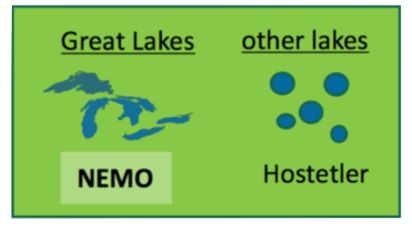
\includegraphics[width=\textwidth]{lake_parameterization_schematic.png}

      \column{0.6\textwidth}
      \begin{itemize}
        \item Horizontal grid size and spacing: 452$\times$260, \textbf{0.1$^\circ$};
        \item Time step:\\ 5 min (\textbf{GEM}); 30 min (\textbf{NEMO});
        \item Surface scheme: \textbf{CLASS3.5}; 1D Lake model: \textbf{Hostetler};
        \item \textbf{NEMO} model is used in the Great Lakes, where \textbf{LIM3} is used for lake ice;
        \item Lateral boundary conditions: ERA-Interim (0.75$^\circ$), CanESM2 (with RCP8.5 emission scenario)
        \end{itemize}
    \end{columns}
  \end{frame}

  \begin{frame}{HLES search algorithm}
  \end{frame}

  \section{HLES in current climate}
  \begin{frame}{Validation: spatial extent}

      \begin{figure}
        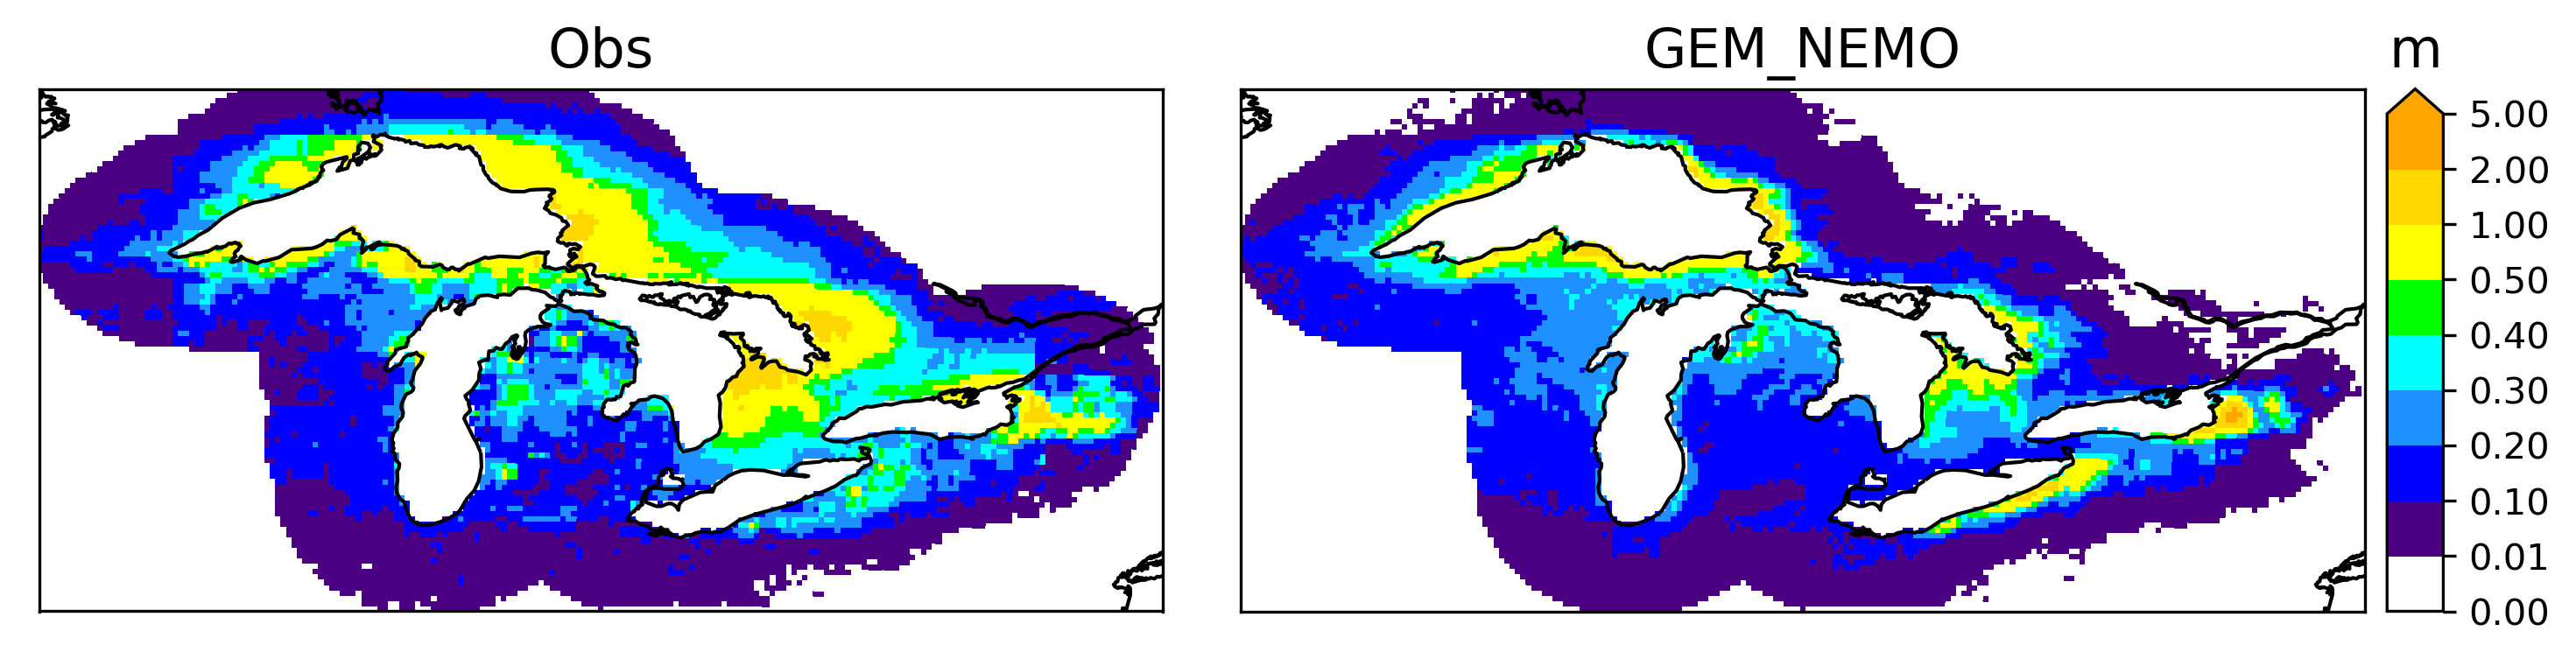
\includegraphics[width=\textwidth]{hles_clim_snow_fall_1980-2009.png}
        \caption{\footnotesize Climatological (1980-2010) yearly HLES (m)}
      \end{figure}

      \begin{itemize}
        \item Extent of HLES is mostly underestimated
        \item Overestimation downwind of lake Erie
        \item Well simulated HLES band extent downwind of lake Ontario, latitude direction
      \end{itemize}
  \end{frame}

  % monthly distribution
  \begin{frame}{Validation: HLES timing}

    \begin{columns}
      \column{0.5\textwidth}
        \begin{figure}
          \includegraphics[height=0.5\textheight]{{hles_histo_all_m9_10_11_12_1_2_3_4_5}.png}
          \caption{\footnotesize Monthly distribution of area-average HLES for the 1980-2010 period}
        \end{figure}

      \column{0.5\textwidth}
        \begin{itemize}
          \item Very good agreement between the model and observations during Nov and Mar
          \item Significant underestimation during Dec and Jan months, probably caused by warm temperature bias
        \end{itemize}


    \end{columns}
  \end{frame}

  \section{Projected changes to HLES}
  \begin{frame}{Projected changes to the fields impacting HLES}
    \begin{tikzpicture}[indicator/.style={scale=0.8, circle, very thick,draw=black!60, minimum size=3.5em}]
        \node (plot) {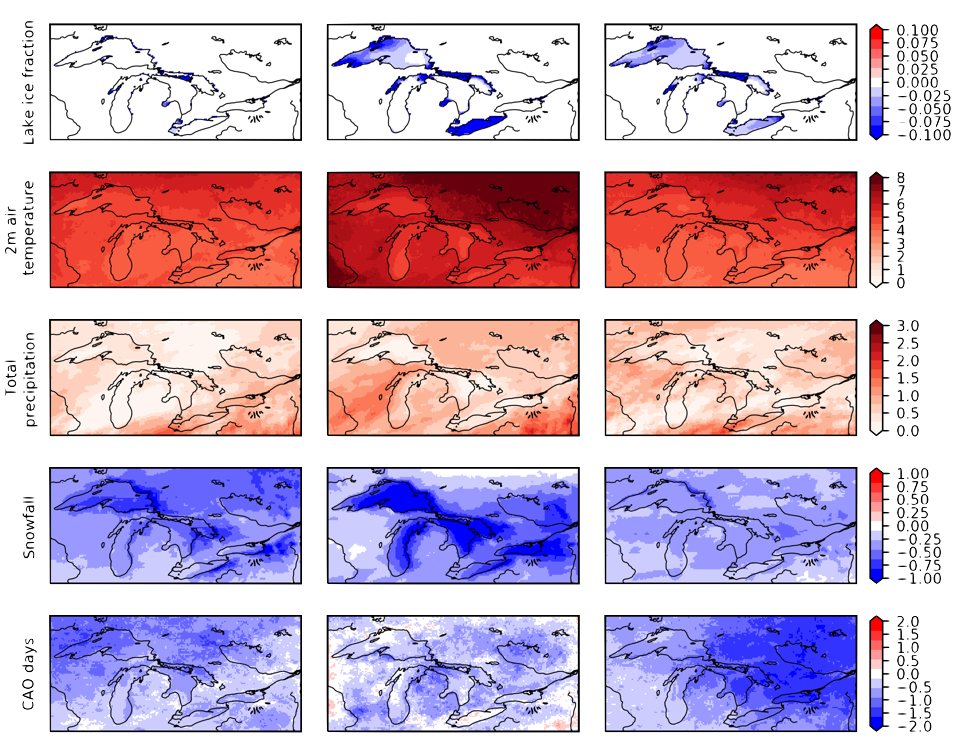
\includegraphics[height=0.85\textheight]{projected_changes_to_surf_and_nearsurf_fields.png}};
        \node[indicator, below right = 1.5em and 0.1em of plot.north east] (icesymbol) {\color{red}{$\pmb+$}};
        \node[indicator, below = 0.8em of icesymbol] (t2msymbol) {\color{blue}{$\pmb-$}\color{black}{/}\color{red}{$\pmb+$}};
        \node[indicator, below = 0.8em of t2msymbol] (prsymbol) {\color{red}{$\pmb+$}};
        \node[indicator, below = 0.8em of prsymbol] (snsymbol) {\color{blue}{$\pmb-$}};
        \node[indicator, below = 0.8em of snsymbol] (caosymbol) {\color{blue}{$\pmb-$}};
        \node[below=0of plot.south]{The signs on the right indicate the impact on the changes to HLES.};
    \end{tikzpicture}

  \end{frame}

  \begin{frame}{Projected changes to HLES: magnitudes and frequencies}
    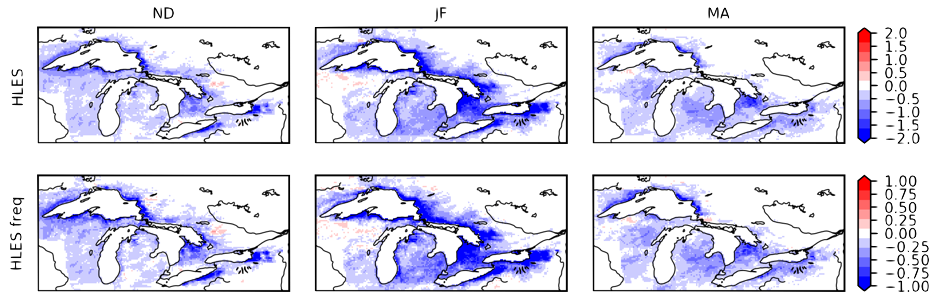
\includegraphics[width=\textwidth]{projected_changes_to_hles.png}
    \begin{itemize}
      \item Mostly decreases up to 1 cm/day
      \item Slight increases south of Lake Superior could be explained by the increased impact of lakes on the dynamics of the atmosphere
    \end{itemize}
  \end{frame}



%% No section here
  \begin{frame}{Conclusions}
    \begin{itemize}
      \item The system shows significant skill in modelling HLES even given resolution limitations.
      \item On average the HLES is projected to be less frequent and of lower intensity in the region.
      \item Slight increase in HLES magnitudes and frequencies is obtained south of Lake Superior during JF months.
      \item Control of ice on the HLES variability is much weaker in the future period.
      \item We need to assess the uncertainty in the HLES derived from observation datasets by using different sources.
    \end{itemize}
  \end{frame}



  \begin{frame}{References}
    \nocite{*}
    \bibliographystyle{apa}
    \bibliography{references}


    todo
    \begin{itemize}
      \item Vavrus et al 2014
      \item GEM/CRCM reference
      \item NEMO reference
    \end{itemize}
  \end{frame}


  \begin{frame}{Acknowledgements}
      \centering
      \Large{Thanks to} \\[\logovspace]
      \small
      \begin{tabular} {m{14em} l}
        \includegraphics[height=1cm]{{nserc_logo}.png} & funding \\[\logovspace]
        \includegraphics[width=10em]{{computecanada_logo}.png}  & computing and storage resources \\[\logovspace]
        \includegraphics[width=5.5em]{{mcgill_logo}.png} \includegraphics[width=4.5em]{{logo_uqam}.png} & base universities   \\[\logovspace]
        \includegraphics[width=14em]{{eccc_logo}.png} & models, libraries and tools \\[\logovspace]
        M. Valin, K. Winger, B. Dugas, F. Dupont and other colleagues & for their help with the project
      \end{tabular}
  \end{frame}


  \begin{frame}[standout]
    Questions?
  \end{frame}

\appendix





\end{document}
